% file: ML.tex
% Machine Learning (notes), in unconventional ``grande'' format; fitting a widescreen format
% 
% github        : ernestyalumni
% gmail         : ernestyalumni 
% linkedin      : ernestyalumni 
% wordpress.com : ernestyalumni
%
% This code is open-source, governed by the Creative Common license.  Use of this code is governed by the Caltech Honor Code: ``No member of the Caltech community shall take unfair advantage of any other member of the Caltech community.'' 

\documentclass[10pt]{amsart}
\pdfoutput=1
\usepackage{mathtools,amssymb,lipsum,caption}

\usepackage{graphicx}
\usepackage{hyperref}
\usepackage[utf8]{inputenc}
\usepackage{listings}
\usepackage[table]{xcolor}
\usepackage{pdfpages}
\usepackage{tikz}
\usetikzlibrary{matrix,arrows}

\usepackage{multicol}

\hypersetup{colorlinks=true,citecolor=[rgb]{0,0.4,0}}

\oddsidemargin=15pt
\evensidemargin=5pt
\hoffset-45pt
\voffset-55pt
\topmargin=-4pt
\headsep=5pt
\textwidth=1120pt
\textheight=595pt
\paperwidth=1200pt
\paperheight=700pt
\footskip=40pt








\newtheorem{theorem}{Theorem}
\newtheorem{corollary}{Corollary}
%\newtheorem*{main}{Main Theorem}
\newtheorem{lemma}{Lemma}
\newtheorem{proposition}{Proposition}

\newtheorem{definition}{Definition}
\newtheorem{remark}{Remark}

\newenvironment{claim}[1]{\par\noindent\underline{Claim:}\space#1}{}
\newenvironment{claimproof}[1]{\par\noindent\underline{Proof:}\space#1}{\hfill $\blacksquare$}

%This defines a new command \questionhead which takes one argument and
%prints out Question #. with some space.
\newcommand{\questionhead}[1]
  {\bigskip\bigskip
   \noindent{\small\bf Question #1.}
   \bigskip}

\newcommand{\problemhead}[1]
  {
   \noindent{\small\bf Problem #1.}
   }

\newcommand{\exercisehead}[1]
  { \smallskip
   \noindent{\small\bf Exercise #1.}
  }

\newcommand{\solutionhead}[1]
  {
   \noindent{\small\bf Solution #1.}
   }


\title{Machine Learning}
\author{Ernest Yeung \href{mailto:ernestyalumni@gmail.com}{ernestyalumni@gmail.com}}
\date{24 avril 2016}
\keywords{Machine Learning, statistical inference, statistical inference learning}
\begin{document}

\definecolor{darkgreen}{rgb}{0,0.4,0}
\lstset{language=C++,
  keywordstyle=\color{blue},
  stringstyle=\color{red},
 commentstyle=\color{darkgreen}
 }
%\lstlistoflistings

\maketitle

\tableofcontents


\begin{multicols*}{2}

\begin{abstract}
Everything about Machine Learning.  
\end{abstract}

\part{Introduction}

\subsubsection{Terminology} \quad \\ 
inputs $\equiv $ independent variables $\equiv $ predictors (cf. statistics) $ \equiv $ features (cf. pattern recognition) \\
outputs $\equiv $ dependent variables $\equiv $ responses

cf. Chapter 2 Overview of Supervised Learning, Section 2.1 Introduction of Hastie, Tibshirani, and Friedman (2009) \cite{HTF2009}

cf. Chapter 2 Overview of Supervised Learning, Section 2.2 Variable Types and Terminology  of Hastie, Tibshirani, and Friedman (2009) \cite{HTF2009}

\subsubsection{$\text{FinSet}$} \quad \\ 
The category $\text{FinSet} \in \mathbf{\text{Cat}}$ is the category of all finite sets (i.e. $\text{Obj}(\text{FinSet}) \equiv $ all finite sets) and all functions in between them; note that $\text{FinSet} \subset \mathbf{\text{Set}}$ \footnote{nlab $\text{FinSet}$ \url{https://ncatlab.org/nlab/show/FinSet}}

Recall that the $\text{FinSet}$ \emph{skeletal} is


\subsection{Supervised Learning}

cf. \url{http://cs229.stanford.edu/notes/cs229-notes1.pdf}

Consider data to belong to the category of all possible data:
\[
\text{Data} \equiv \text{Dat} = (\text{Obj}(\text{Dat}), \text{Mor}\text{Dat}, 1, \circ), \qquad \, \text{Dat} \in \mathbf{\text{Cat}}
\]
Consider the \textbf{training set}:
\[
\text{training set} := \lbrace (x^{(i)},y^{(i)}) | i  =1 \dots m , x^{(i)} \in \mathcal{X}, y^{(i)} \in \mathcal{Y} \rbrace
\]
where $\mathcal{X}$ is a manifold (it can be topological or smooth, EY:20160502 I don't know exactly because I need to check the topological and/or differential structure); $\mathcal{Y} \in \text{Obj}(\text{FinSet})$, or $(\mathcal{Y} \in \text{Obj}(\text{Top}) (\text{or } \mathcal{Y} \in \text{Obj}(\text{Man})))$.  

So training set $ \subset \mathcal{X} \times \mathcal{Y} \in \text{Obj}(\text{Dat})$.  

I propose that there should be a functor $H$ that represents the ``learning algorithm'':
\[
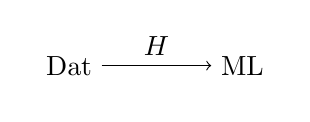
\begin{tikzpicture}
  \matrix (m) [matrix of math nodes, row sep=3em, column sep=4em, minimum width=2em]
  {
\text{Dat} & \text{ML}  \\
};
  \path[->]
  (m-1-1) edge node [above] {$H$} (m-1-2)
  ;
\end{tikzpicture}
\]
s.t.
\[
\begin{aligned}
  & H:\mathcal{X}\times \mathcal{Y} \to \text{Hom}(\mathcal{X}, \mathcal{Y}) \\ 
  & H(\text{training set}) = H(\lbrace (x^{(i)},y^{(i)} )| i  =1 \dots m \rbrace) = h 
\end{aligned}
\]

When $\mathcal{Y} \in \text{Obj}(\text{FinSet})$, \emph{classification}. \\
When $\mathcal{Y} \in \text{Obj}(\text{Top})$ (or $\text{Obj}(\text{Man})$, \emph{regression}.

\subsubsection{Linear Regression}

Keeping in mind   
\[
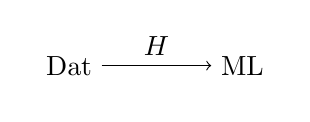
\begin{tikzpicture}
  \matrix (m) [matrix of math nodes, row sep=3em, column sep=4em, minimum width=2em]
  {
\text{Dat} & \text{ML}  \\
};
  \path[->]
  (m-1-1) edge node [above] {$H$} (m-1-2)
  ;
\end{tikzpicture}
\]
Consider \[
\begin{aligned}
  & h:\mathbb{R}^p \to \text{Hom}(\mathcal{X},\mathcal{Y}) \\ 
  & h:\theta \mapsto h_{\theta} 
\end{aligned}
\]
s.t. 
\[
h_{\theta} : \mathcal{X} \to \mathcal{Y}
\]
so (possibly) $h\in \text{Obj}ML$ (or is $h$ part of the functor $H$?)

Consider the cost function $J$
\[
\begin{aligned}
  & J:\mathbb{R}^p \to \text{Hom}(\mathfrak{X}\times \mathfrak{Y}, \mathbb{R}) = C^{\infty}(\mathcal{X}\times \mathcal{Y}) \\ 
  & J(\theta) = \frac{1}{2} \sum_{i=1}^m (h_{\theta}(x^{(i)}) - y^{(i)})^2 
\end{aligned}
\]

\subsubsection{LMS algorithm (least mean square (or Widrow-Hoff learning rule))}

Define \textbf{gradient descent} algorithm:
\[
\theta_j := \theta_j- \alpha \frac{ \partial }{ \partial \theta_j} J(\theta)
\]
with $:=$ being assignment (I'll use $:=$ for ``define'', in mathematical terms, use context to distinguish the 2), where $\alpha$ is the \emph{learning rate}.  

Rewriting the above,
\[
\theta := \theta - \alpha \text{grad}J(\theta)
\]
where $\text{grad} : C^{\infty}(M) \to \mathfrak{X}(M)$, with $M$ being a smooth manifold.  

This is \emph{batch gradient descent}:
\[
\begin{gathered}
  \theta_j := \theta_j -\alpha \frac{ \partial }{ \partial \theta_j} J(\theta) = \theta_j - \alpha \frac{ \partial }{ \partial \theta_j} \frac{1}{2} \sum_{i=1}^m ( h_{\theta}(x^{(i)}) - y^{(i)})^2  = \theta_j - \alpha \sum_{i=1}^m (h_{\theta}(x^{(i)}) - y^{(i)} ) \left( \frac{ \partial h_{\theta}(x^{(i)}) }{\partial \theta} \right)
\end{gathered}
\]
Simply notice how the entire training set of $m$ rows is used.  

I will expound on the so-called distinguished object $1\xrightarrow{P}X$ on pp. 8, in Section 2 The Category of Conditional Probabilities of Culbertson and Sturtz (2013) \cite{CS2013} because it wasn't clear to me in the first place (the fault is mine; the authors wrote a very lucid and very fathomable, pedagogically-friendly exposition).  

$\forall \, Y $ with indiscrete $\sigma$-algebra $\Sigma_Y = \lbrace Y ,\emptyset \rbrace$ \\
\phantom{ \qquad \, } (remember, $((Y,\Sigma_Y), \mu_Y)$, $\mu_Y(\phi) = 0$, $\mu_Y(Y)=1$), \\
\qquad \\ 
$\exists \, !$ unique morphism in $\text{Mor}\mathcal{P}$, $X\to Y$, since 

$\forall \, P:X\to Y$, $P \in \text{Mor}\mathcal{P}$, $P_x$ must be a probability measure on $Y$, because 
\[
\begin{gathered}
  (X,\Sigma_X) \xrightarrow{ P } (Y,\Sigma_Y) \\ 
  P:\Sigma_Y\times X \to [0,1] \\ 
  P(\cdot | x):\Sigma_Y \to [0,1] \equiv \begin{gathered} P_x:\Sigma_Y \to [0,1]  \text{ s.t. }  \\ P_x(\emptyset) =0, \, P_x(Y) =1 \end{gathered}
\end{gathered}
\]
i.e. EY: 20160503, Given $x\in X$ occurs, $Y$ must occur. 

By def. of terminal object ($\forall \, (X,\Sigma_X) \in \text{Obj}\mathcal{P}$, $\exists \, !$ morphism $P$ s.t. $(X,\Sigma_X) \xrightarrow{P} (Y,\Sigma_Y)$, \\
$Y$ \emph{terminal} object, and denote unique morphism $!_X : X\to Y$, $!_X \in \text{Mor}\mathcal{P}$.  

Up to isomorphism, canonical terminal object is 1-element set denoted by $1 = \lbrace * \rbrace$, with the only possible $\sigma$-algebra ($\mu(*)=1, \, \mu(\emptyset) = 0$),

\[
\forall \, P:1 \to X, \, P\in \text{Mor}\mathcal{P}, \, P \in \text{Hom}_{\mathcal{P}}(1,X) , \, \forall \, X \in \text{Mor}\mathcal{P}
\]
$P$ is an ``absolute'' probability measure on $X$ because ``there's no variability (conditioning) possible within singleton set $1 = \lbrace * \rbrace$.''  \cite{CS2013}

Now
\[
\begin{aligned}
  & P:\Sigma_X \times 1 \to [0,1] \\ 
  & P(\cdot | *) : \Sigma_X \to [0,1]
\end{aligned}
\]
where $P(\cdot | *) : \Sigma_X \to [0,1]$ perfect probability measure on $X$, $P(\cdot | *) : \Sigma_X \to [0,1] \equiv P_*$, i.e. $P(\cdot | *) = p(\cdot )$ (usual probability on $X$).  

$\forall \, A \in \Sigma_X$, $P(A|\cdot ) : 1 \to [ 0,1]$, but $P(A|*) = P(A)$, $P(A|\emptyset ) = 0$.  

Refer to 
\[
1\xrightarrow{P} X
\]
morphism $P:1\to X \in \text{Mor}\mathcal{P}$ as probability measure or distribution on $X$.  




\section{Parallel Computing}

\subsection{Udacity Intro to Parallel Programming : Lesson 1 - The GPU Programming Model}

Owens and Luebki pound fists at the end of this video.  $=))))$  \href{https://classroom.udacity.com/courses/cs344/lessons/55120467/concepts/658304810923}{Intro to the class}.

\subsubsection{Running CUDA locally}
Also, \href{https://classroom.udacity.com/courses/cs344/lessons/55120467/concepts/658304810923}{Intro to the class}, in Lesson 1 - The GPU Programming Model, has links to documentation for running CUDA locally; in particular, for Linux: \url{http://docs.nvidia.com/cuda/cuda-getting-started-guide-for-linux/index.html}.  That guide told me to go download the NVIDIA CUDA Toolkit, which is the \href{NVIDIA CUDA Developer Toolkit}{https://developer.nvidia.com/cuda-downloads}.  

For \emph{Fedora}, I chose Installer Type \verb|runfile (local)|.  

Afterwards, installation of CUDA on Fedora 23 workstation had been nontrivial.  Go see either my github repository \href{https://github.com/ernestyalumni/MLgrabbag/blob/master/README.md}{MLgrabbag} (which will be updated) or my \href{https://ernestyalumni.wordpress.com/2016/05/07/fedora-23-workstation-linuxnvidia-geforce-gtx-980-ti-my-experience-log-of-what-i-do-and-find-out/#CUDAinstall}{wordpress blog} (which may not be upgraded frequently).  


$P=VI = I^2R$ heating.

\subsubsection{Definitions of Latency and throughput (or bandwidth)}

cf. 
\href{https://classroom.udacity.com/courses/cs344/lessons/55120467/concepts/669874580923}{Building a Power Efficient Processor}

\href{https://classroom.udacity.com/courses/cs344/lessons/55120467/concepts/667559300923}{Latency vs Bandwidth}

latency $[\text{sec}]$.  From the title ``Latency vs. bandwidth'', I'm thinking that throughput $=$ bandwidth (???).  throughput $ = $ job$/$time (of job).  

Given total task, velocity $v$, \\
total task $/v = $ latency.  throughput $=$ latency$/(\text{jobs per total task})$.  


Also, in \href{https://classroom.udacity.com/courses/cs344/lessons/55120467/concepts/669874580923}{Building a Power Efficient Processor}.  Owens recommends the article David Patterson, ``Latency...''

cf. \href{https://classroom.udacity.com/courses/cs344/lessons/55120467/concepts/671181630923}{GPU from the Point of View of the Developer}

$n_{\text{core}} \equiv $ number of cores \\
$n_{\text{vecop}} \equiv$ ($n_{\text{vecop}}-$wide axial vector operations$/core$ core) \\
$n_{\text{thread}} \equiv $ threads$/$core (hyperthreading)
\[
n_{\text{core}} \cdot n_{\text{vecop}} \cdot n_{\text{thread}}  \text{ parallelism  }
\]

There were various websites that I looked up to try to find out the capabilities of my video card, but so far, I've only found these commands (and I'll print out the resulting output):
{\scriptsize
\begin{lstlisting}
$ lspci -vnn | grep VGA -A 12
03:00.0 VGA compatible controller [0300]: NVIDIA Corporation GM200 [GeForce GTX 980 Ti] [10de:17c8] (rev a1) (prog-if 00 [VGA controller])
	Subsystem: eVga.com. Corp. Device [3842:3994]
	Physical Slot: 4
	Flags: bus master, fast devsel, latency 0, IRQ 50
	Memory at fa000000 (32-bit, non-prefetchable) [size=16M]
	Memory at e0000000 (64-bit, prefetchable) [size=256M]
	Memory at f0000000 (64-bit, prefetchable) [size=32M]
	I/O ports at e000 [size=128]
	[virtual] Expansion ROM at fb000000 [disabled] [size=512K]
	Capabilities: <access denied>
	Kernel driver in use: nvidia
	Kernel modules: nouveau, nvidia

$ lspci | grep VGA -E
03:00.0 VGA compatible controller: NVIDIA Corporation GM200 [GeForce GTX 980 Ti] (rev a1)

$ grep driver /var/log/Xorg.0.log
[    18.074] Kernel command line: BOOT_IMAGE=/vmlinuz-4.2.3-300.fc23.x86_64 root=/dev/mapper/fedora-root ro rd.lvm.lv=fedora/root rd.lvm.lv=fedora/swap rhgb quiet LANG=en_US.UTF-8 nouveau.modeset=0 rd.driver.blacklist=nouveau nomodeset gfxpayload=vga=normal
[    18.087] (WW) Hotplugging is on, devices using drivers 'kbd', 'mouse' or 'vmmouse' will be disabled.
[    18.087] 	X.Org XInput driver : 22.1
[    18.192] (II) Loading /usr/lib64/xorg/modules/drivers/nvidia_drv.so
[    19.088] (II) NVIDIA(GPU-0): Found DRM driver nvidia-drm (20150116)
[    19.102] (II) NVIDIA(0):     ACPI event daemon is available, the NVIDIA X driver will
[    19.174] (II) NVIDIA(0): [DRI2]   VDPAU driver: nvidia
[    19.284] 	ABI class: X.Org XInput driver, version 22.1
...

$ lspci -k | grep -A 8 VGA
03:00.0 VGA compatible controller: NVIDIA Corporation GM200 [GeForce GTX 980 Ti] (rev a1)
	Subsystem: eVga.com. Corp. Device 3994
	Kernel driver in use: nvidia
	Kernel modules: nouveau, nvidia
03:00.1 Audio device: NVIDIA Corporation GM200 High Definition Audio (rev a1)
	Subsystem: eVga.com. Corp. Device 3994
	Kernel driver in use: snd_hda_intel
	Kernel modules: snd_hda_intel
05:00.0 USB controller: VIA Technologies, Inc. VL805 USB 3.0 Host Controller (rev 01)
  \end{lstlisting}
}
\href{https://classroom.udacity.com/courses/cs344/lessons/55120467/concepts/671181640923}{CUDA Program Diagram}

\[
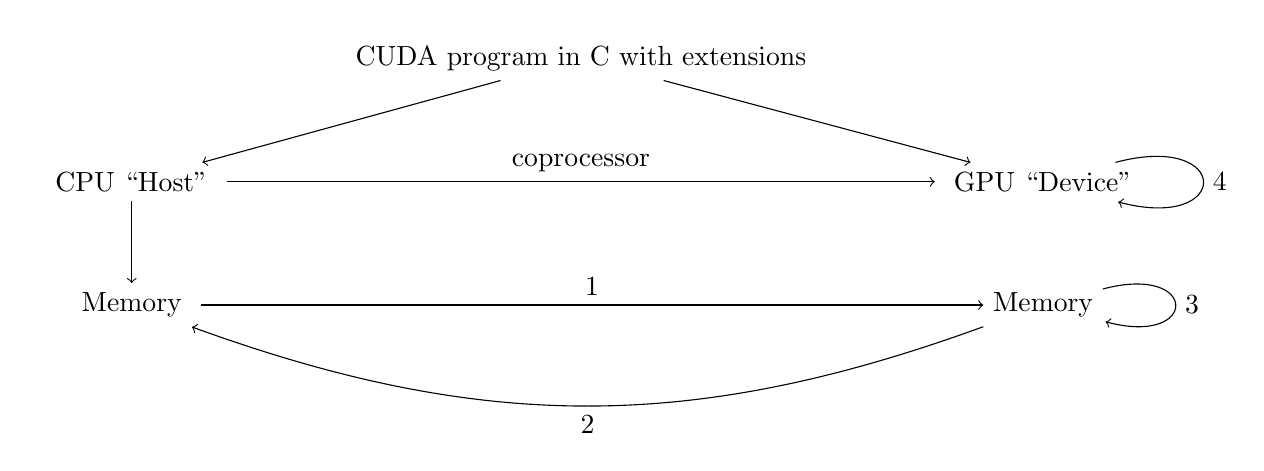
\begin{tikzpicture}
  \matrix (m) [matrix of math nodes, row sep=3em, column sep=4em, minimum width=1em]
  {
    & \text{ CUDA program in C with extensions } &  \\
    \text{ CPU ``Host'' } & & \text{ GPU ``Device'' } \\
    \text{ Memory } & & \text{Memory} \\
};
  \path[->]
  (m-1-2) edge node [above] {} (m-2-1)
  edge node [above] {} (m-2-3)
  (m-2-1) edge node [above] { coprocessor } (m-2-3)
  edge node [above] {} (m-3-1)
  (m-3-1) edge node [above] {$1$} (m-3-3)
  (m-3-3) edge [bend left=20] node [below] {$2$} (m-3-1)
  edge [loop right] node [right] {$3$} (m-3-3)
  (m-2-3) edge [loop right] node [right] {$4$} (m-2-3)
  ;
\end{tikzpicture}
\]
CPU ``host'' is the boss (and issues commands) -Owen.

$\text{Coprocessor} : \text{ CPU ``host'' } \to \text{ GPU ``device'' } $ \\
$\text{Coprocessor} : \text{ CPU process } \mapsto \text{ (co)-process out to GPU } $ \\

With
\begin{enumerate}
  \item[1] data cpu $\to $ gpu
  \item[2] data gpu $\to$ cpu \qquad (initiated by cpu host) \\

$1.,2.,$ uses \verb|cudaMemcpy| 
  \item[3] allocate GPU memory: \verb|cudaMalloc|
  \item[4] launch kernel on GPU
  \end{enumerate}
Remember that for 4., this launching of the kernel, while it's acting on GPU ``device'' onto itself, it's initiated by the boss, the CPU ``host''.

Hence, cf. \href{https://classroom.udacity.com/courses/cs344/lessons/55120467/concepts/670489380923}{Quiz: What Can GPU Do in CUDA}, GPUs can respond to CPU request to receive and send Data CPU $\to $ GPU and Data GPU $\to $ CPU, respectively (1,2, respectively), and compute a kernel launched by the CPU (3).


\href{https://classroom.udacity.com/courses/cs344/lessons/55120467/concepts/670742800923}{A CUDA Program}
A typical GPU program

\begin{itemize}
\item \verb|cudaMalloc| - CPU allocates storage on GPU 
\item \verb|cudaMemcpy| - CPU copies input data from CPU $\to $ GPU 
\item \emph{kernel launch} - CPU launches kernel(s) on GPU to process the data 
\item \verb|cudaMemcpy| - CPU copies results back to CPU from GPU
  \end{itemize}

Owens advises minimizing ``communication'' as much as possible (e.g. the \verb|cudaMemcpy| between CPU and GPU), and do a lot of computation in the CPU and GPU, each separately.

\href{https://classroom.udacity.com/courses/cs344/lessons/55120467/concepts/672300540923}{Defining the GPU Computation}

Owens circled this
{\Large
  \[
  \begin{gathered}
\text{ BIG IDEA } \qquad \, \boxed{ \text{ This is Important } }  \\
\begin{aligned} 
& \text{ Kernels look like serial programs } \\
  & \text{ Write your program as if it will run on \textbf{ one } thread } \\
  & \text{The GPU will run that program on \textbf{ many } threads}
  \end{aligned}
\end{gathered}
\]
}

\href{https://classroom.udacity.com/courses/cs344/lessons/55120467/concepts/670742840923}{Squaring A Number on the CPU}

Note
\begin{enumerate}
\item Only 1 thread of execution: (``thread'' $:=$ one independent path of execution through the code) e.g. the \verb|for| loop
  \item no explicit parallelism; it's serial code e.g. the \verb|for| loop through 64 elements in an array
  \end{enumerate}


\href{https://classroom.udacity.com/courses/cs344/lessons/55120467/concepts/670742870923}{GPU Code A High Level View}

CPU:
\begin{itemize}
  \item Allocate Memory 
  \item Copy Data to/from GPU
    \item Launch Kernel - species degree of parallelism
\end{itemize}

GPU:
\begin{itemize}
\item Express Out $=$ In $\cdot $ In  - says \emph{nothing} about the degree of parallelism
  \end{itemize}

Owens reiterates that in the GPU, everything looks serial, but it's only in the CPU that anything parallel is specified.  

pseudocode: CPU code: square kernel $<<< 64 >>>$ (outArray,inArray)

\href{https://classroom.udacity.com/courses/cs344/lessons/55120467/concepts/670742940923}{Squaring Numbers Using CUDA Part 3}

From the example
\begin{lstlisting}
  // launch the kernel
  square<<<1, ARRAY_SIZE>>>(d_out, d_in)
  \end{lstlisting}
we're introduced to the ``CUDA launch operator'', initiating a kernel of 1 block of 64 elements (\verb|ARRAY_SIZE| is 64) on the GPU.  Remember that \verb|d_| prefix (this is naming comvention) tells us it's on the device, the GPU, solely.  

With CUDA launch operator $\equiv <<<>>>$, then also looking at this explanation on \verb|stackexchange| (so surely others are confused as well, of those who are learning this (cf. \href{http://stackoverflow.com/questions/19240658/cuda-kernel-launch-parameters-explained-right}{CUDA kernel launch parameters explained right?}).  From \href{http://stackoverflow.com/users/1957265/eric}{Eric}'s answer, \\

threads are grouped into blocks.  all the threads will execute the invoked kernel function.

Certainly,
\[
\begin{aligned}
  & <<<>>>:(n_{\text{block}}, n_{\text{threads}})\times \text{kernelfunctions} \mapsto \text{kernelfunction}<<<n_{\text{block}},n_{\text{threads}}>>> \in \text{End}:\text{Dat}_{\text{GPU}} \\ 
  & <<<>>>: \mathbb{N}^+ \times \mathbb{N}^+ \times \text{Mor}_{\text{GPU}} \to \text{End}\text{Dat}_{\text{GPU}}
  \end{aligned}
\]
where I propose that GPU can be modeled as a category containing objects $\text{Dat}_{\text{GPU}}$, the collection of all possible data inputs and outputs into the GPU, and $\text{Mor}_{\text{GPU}}$, the collection of all kernel functions that run (exclusively, and this \emph{must} be the class, as reiterated by Prof. Owen) on the GPU.

Next,
\[
\begin{aligned}
  & \text{kernelfunction}<<<n_{\text{block}},n_{\text{threads}}>>>: \text{din}\mapsto \text{dout} \qquad \, (\text{as given in the ``square'' example, and so I propose}) \\ 
  & \text{kernelfunction}<<<n_{\text{block}},n_{\text{threads}}>>>:(\mathbb{N}^+)^{n_{\text{threads}}} \to (\mathbb{N}^+)^{n_{\text{threads}}}
  \end{aligned}
\]
But keep in mind that $\text{dout}$, $\text{din}$ are pointers in the C program, pointers to the place in the memory.  

\verb|cudaMemcopy| is a functor category, s.t. e.g. $\text{Obj}_{\text{CudaMemcopy}} \ni \text{cudaMemcpyDevicetoHost}$ where
\[
\text{cudaMemcopy}(-,-,n_{\text{thread}},\text{cudaMemcpyDeviceToHost}): \text{Memory}_{\text{GPU}} \to \text{Memory}_{\text{CPU}} \in \text{Hom}(\text{Memory}_{\text{GPU}}, \text{Memory}_{\text{CPU}})
\]

\href{https://classroom.udacity.com/courses/cs344/lessons/55120467/concepts/670742910923}{Squaring Numbers Using CUDA 4}

Note the C language construct \emph{declaration specifier} - denotes that this is a kernel (for the GPU) and not CPU code.  Pointers need to be allocated on the GPU (otherwise your program will crash spectacularly -Prof. Owen).  

\subsubsection{What are C pointers?}

Is $\langle \text{ type } \rangle \, *$, a pointer, then a mapping from the category, namely the objects of types, to a mapping from the specified value type to a memory address?

e.g.
\[
\begin{aligned}
  \langle \, \rangle \, * & : \text{float} \mapsto \text{float} \, * \\ 
  \text{float } \, * & : \text{din} \mapsto \text{ some memory address }
\end{aligned}
\]
and then we pass in mappings, not values, and so we're actually declaring a square \emph{functor}.

What is \verb|threadIdx|?  What is it mathematically?  Consider that $\exists \,$ 3 ``modules'':

\[
\begin{aligned}
  & \text{threadIdx}.x \\
  & \text{threadIdx}.y \\
  & \text{threadIdx}.z 
\end{aligned}
\]
And then the line
\begin{lstlisting}
int idx = threadIdx.x;
  \end{lstlisting}
says that idx is an integer, ``declares'' it to be so, and then assigns idx to $\text{threadIdx}.x$ which surely has to also have the same type, integer.  So (perhaps)
\[
idx \equiv \text{threadIdx}.x \in \mathbb{Z}
\]
is the same thing.

Then suppose threadIdx $\subset \mathbf{\text{FinSet}}$, a subcategory of the category of all (possible) finite sets, s.t. threadIdx has 3 particular morphisms, $x,y,z\in \text{Mor}threadIdx$,
\[
\begin{aligned}
  & x : \text{threadIdx} \mapsto \text{threadIdx}.x \in \text{Obj}_{\mathbf{\text{FinSet}}} \\ 
  & y : \text{threadIdx} \mapsto \text{threadIdx}.x \in \text{Obj}_{\mathbf{\text{FinSet}}} \\ 
  & z : \text{threadIdx} \mapsto \text{threadIdx}.x \in \text{Obj}_{\mathbf{\text{FinSet}}}  
\end{aligned}
\]

\href{https://classroom.udacity.com/courses/cs344/lessons/55120467/concepts/670742980923}{Configuring the Kernel Launch Parameters Part 1}

$n_{\text{blocks}}$, $n_{\text{threads}}$ with $n_{\text{threads}} \geq 1024$ (this maximum constant is GPU dependent).  You should pick the $(n_{\text{blocks}}, n_{\text{threads}})$ that makes sense for your problem, says Prof. Owen.  

\subsubsection{Memory layout of blocks and threads}

$\forall \, (n_{\text{blocks}}, n_{\text{threads}}) \in \mathbb{Z} \times \lbrace 1 \dots 1024 \rbrace$, $\lbrace 1 \dots n_{\text{block}} \times \lbrace 1 \dots n_{\text{threads}} \rbrace$ is now an ordered index (with lexicographical ordering).  This is just 1-dimensional (so possibly there's a 1-to-1 mapping to a finite subset of $\mathbb{Z}$).

I propose that ``adding another dimension'' or the 2-dimension, that Prof. Owen mentions is being able to do the Cartesian product, up to 3 Cartesian products, of the block-thread index.  

\href{https://classroom.udacity.com/courses/cs344/lessons/55120467/concepts/668398860923}{Quiz: Configuring the Kernel Launch Parameters 2 }

Most general syntax:

Configuring the kernel launch
\begin{lstlisting}
  kernel<<<grid of blocks, block of threads >>>(...)

  // for example

  square<<<dim3(bx,by,bz), dim3(tx,ty,tz), shmem>>>(...)
  \end{lstlisting}
where \verb|dim3(tx,ty,tz)| is the grid of blocks $bx\cdot by \cdot bz$ \\
\phantom{ where } \verb|{dim3}(tx,ty,tz)| is the block of threads $tx \cdot ty \cdot tz$ \\
\phantom{ where } \verb|shmem| is the shared memory per block in bytes


\href{https://classroom.udacity.com/courses/cs344/lessons/55120467/concepts/967066740923}{Problem Set 1}
``Also, the image is represented as an 1D array in the kernel, not a 2D array like I mentioned in the video.''

Here's part of that code for squaring numbers:
\begin{lstlisting}
  __global__ void square(float *d_out, float *d_in) {
    int idx = threadIdx.x;
    float f = d_in[idx];
    d_out[idx] = f*f;
    }
  \end{lstlisting}

\subsubsection{Grid of blocks, block of threads, thread that's indexed; (mathematical) structure of it all}

Let
\[
\begin{gathered}
  \text{grid} = \prod_{I=1}^N (\text{block})^{n_I^{\text{block}}}
\end{gathered}
\]
where $N=1,2,3$ (for CUDA) and by naming convention $\begin{aligned} & \quad \\
  & I = 1 \equiv x \\
  & I = 2 \equiv y \\
  & I = 3 \equiv z \end{aligned}$

Let's try to make it explicity (as others had difficulty understanding the grid, block, thread model, cf. \href{http://stackoverflow.com/questions/14711668/colored-image-to-greyscale-image-using-cuda-parallel-processing}{colored image to greyscale image using CUDA parallel processing}, \href{http://stackoverflow.com/questions/16619274/cuda-griddim-and-blockdim}{Cuda gridDim and blockDim}) through commutative diagrams and categories (from math):

\[
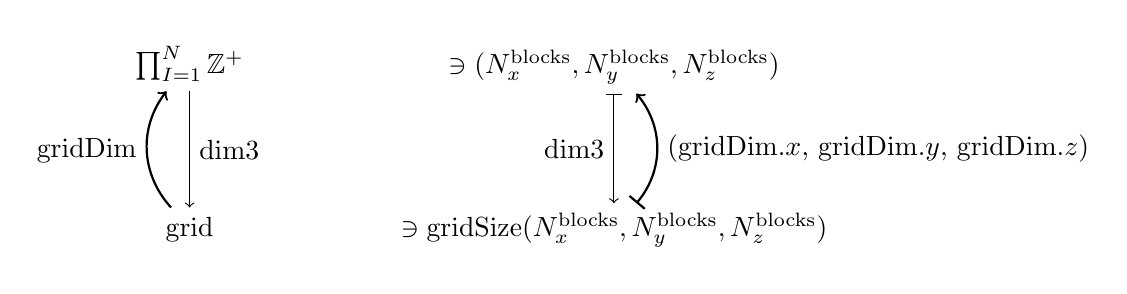
\begin{tikzpicture}
  \matrix (m) [matrix of math nodes, row sep=4em, column sep=5em, minimum width=2em]
  {
\prod_{I=1}^N \mathbb{Z}^+ & \ni (N_x^{\text{blocks}}, N_y^{\text{blocks}} , N_z^{\text{blocks}}) \\
\text{grid} & \ni \text{gridSize}(N_x^{\text{blocks}}, N_y^{\text{blocks}} , N_z^{\text{blocks}} ) \\
};
  \path[->]
  (m-1-1) edge node [right] {$\text{dim}3$} (m-2-1)
  (m-2-1) edge [bend left=40, thick] node [left] {$\text{gridDim}$} (m-1-1)
  ;
  \path[|->]
  (m-1-2) edge node [left] {$\text{dim}3$} (m-2-2)
  (m-2-2) edge [bend right=40, thick] node [right] {$(\text{gridDim}.x$, $\text{gridDim}.y$, $\text{gridDim}.z)$} (m-1-2)
  ;  
\end{tikzpicture}
\]

\[
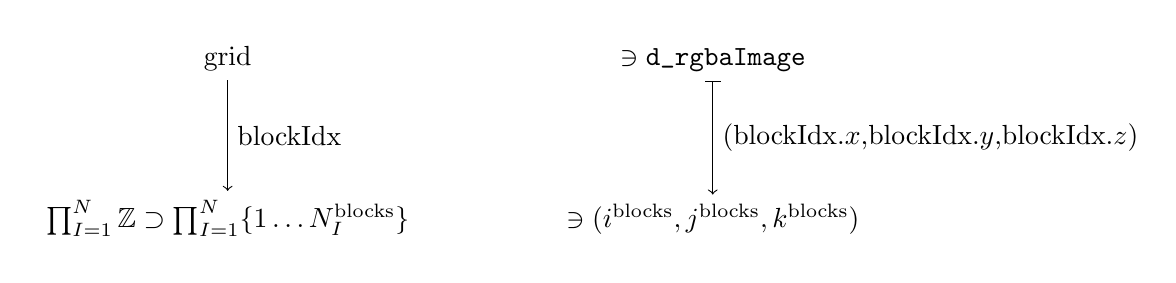
\begin{tikzpicture}
  \matrix (m) [matrix of math nodes, row sep=4em, column sep=5em, minimum width=2em]
  {
    \text{grid} & \ni \verb|d_rgbaImage| \\
    \prod_{I=1}^N \mathbb{Z} \supset \prod_{I=1}^N \lbrace 1 \dots N_I^{\text{blocks}} \rbrace & \ni (i^{\text{blocks}},j^{\text{blocks}}, k^{\text{blocks}} ) \\
};
  \path[->]
  (m-1-1) edge node [right] {$\text{blockIdx}$} (m-2-1)
  ;
  \path[|->]
  (m-1-2) edge node [right] {($\text{blockIdx}.x$,$\text{blockIdx}.y$,$\text{blockIdx}.z$)} (m-2-2)
  ;
  \end{tikzpicture}
\]

and then similar relations (i.e. arrows, i.e. relations) go for a block of threads:

\[
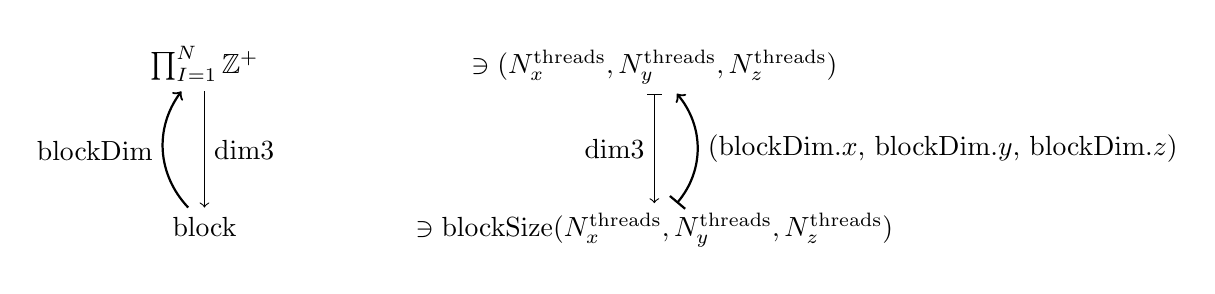
\begin{tikzpicture}
  \matrix (m) [matrix of math nodes, row sep=4em, column sep=5em, minimum width=2em]
  {
\prod_{I=1}^N \mathbb{Z}^+ & \ni (N_x^{\text{threads}}, N_y^{\text{threads}} , N_z^{\text{threads}}) \\
\text{block} & \ni \text{blockSize}(N_x^{\text{threads}}, N_y^{\text{threads}} , N_z^{\text{threads}} ) \\
};
  \path[->]
  (m-1-1) edge node [right] {$\text{dim}3$} (m-2-1)
  (m-2-1) edge [bend left=40, thick] node [left] {$\text{blockDim}$} (m-1-1)
  ;
  \path[|->]
  (m-1-2) edge node [left] {$\text{dim}3$} (m-2-2)
  (m-2-2) edge [bend right=40, thick] node [right] {$(\text{blockDim}.x$, $\text{blockDim}.y$, $\text{blockDim}.z)$} (m-1-2)
  ;  
\end{tikzpicture}
\]

\[
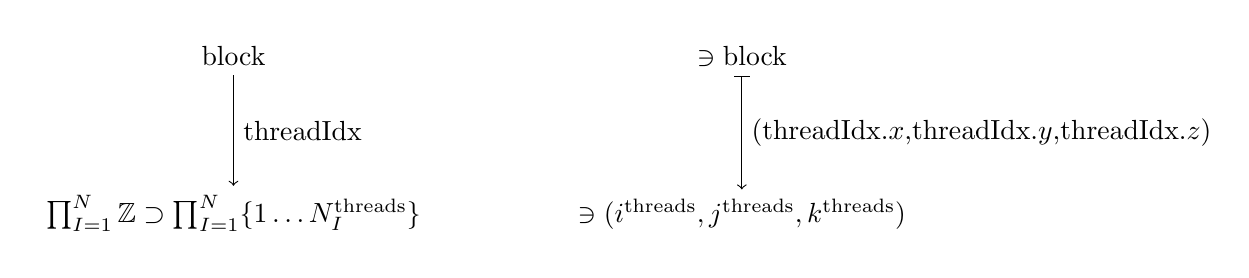
\begin{tikzpicture}
  \matrix (m) [matrix of math nodes, row sep=4em, column sep=5em, minimum width=2em]
  {
    \mathbf{\text{block}} & \ni \text{block} \\
    \prod_{I=1}^N \mathbb{Z} \supset \prod_{I=1}^N \lbrace 1 \dots N_I^{\text{threads}} \rbrace & \ni (i^{\text{threads}},j^{\text{threads}}, k^{\text{threads}} ) \\
};
  \path[->]
  (m-1-1) edge node [right] {$\text{threadIdx}$} (m-2-1)
  ;
  \path[|->]
  (m-1-2) edge node [right] {($\text{threadIdx}.x$,$\text{threadIdx}.y$,$\text{threadIdx}.z$)} (m-2-2)
  ;
  \end{tikzpicture}
\]

\href{https://discussions.udacity.com/t/gridsize-help-assignment-1-pp/124701}{gridsize help assignment 1 Pp} explains how threads per block is variable, and remember how Owens said Luebki says that a GPU doesn't get up for more than a 1000 threads per block.  

\subsubsection{Generalizing the model of an image}

Consider vector space $V$, e.g. $\text{dim}V=4$, vector space $V$ over field $\mathbb{K}$, so $V= \mathbb{K}^{\text{dim}V}$.

Each pixel represented by $\forall \, v \in V$.

Consider an image, or space, $M$.  $\text{dim}M = 2$ (image), $\text{dim}M=3$.  Consider a local chart (that happens to be global in our case):
\[
\begin{aligned}
  & \varphi : M \to \mathbb{Z}^{\text{dim}M} \supset \lbrace 1 \dots N_1 \rbrace \times \lbrace 1 \dots N_2 \rbrace \times \dots \times \lbrace 1 \dots N_{\text{dim}M} \rbrace \\ 
  & \varphi : x \mapsto (x^1(x), x^2(x), \dots , x^{\text{dim}M}(x) )
  \end{aligned}
\]
\[
\begin{tikzpicture}
  \matrix (m) [matrix of math nodes, row sep=4em, column sep=5em, minimum width=2em]
  {
    E & M \times V \\ 
    M &  \\
};
  \path[->]
  (m-1-1) edge node [auto] {$\varphi$} (m-1-2)
          edge node [left] {$\pi$} (m-2-1)
  (m-1-2) edge node [auto] {$$} (m-2-1)
              ;
  \end{tikzpicture}
\qquad \, 
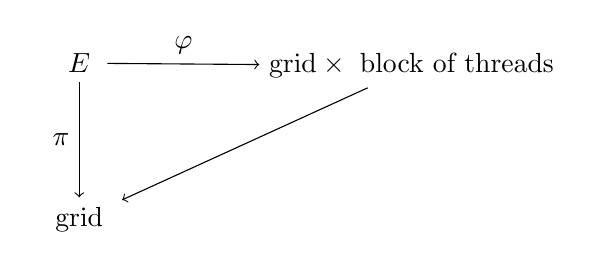
\begin{tikzpicture}
  \matrix (m) [matrix of math nodes, row sep=4em, column sep=5em, minimum width=2em]
  {
    E & \text{grid} \times \text{ block of threads } \\ 
    \text{ grid } & \\
};
  \path[->]
  (m-1-1) edge node [auto] {$\varphi$} (m-1-2)
          edge node [left] {$\pi$} (m-2-1)
  (m-1-2) edge node [auto] {$$} (m-2-1)
              ;
  \end{tikzpicture}
\]

Consider a ``coarsing'' of underlying $M$:
\[
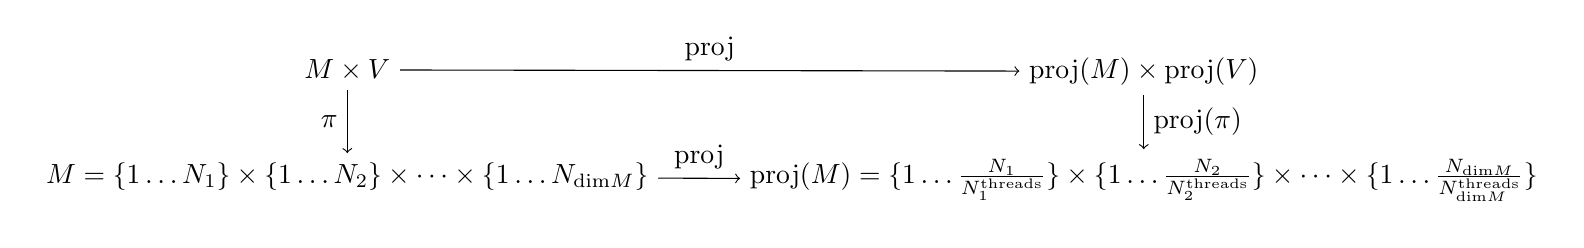
\begin{tikzpicture}
  \matrix (m) [matrix of math nodes, row sep=2em, column sep=3em, minimum width=1em]
  {
    M\times V & \text{proj}(M) \times \text{proj}(V) \\ 
    M = \lbrace 1 \dots N_1 \rbrace \times \lbrace 1 \dots N_2 \rbrace \times \dots \times \lbrace 1 \dots N_{\text{dim}M} \rbrace  & \text{proj}(M)  = \lbrace 1 \dots \frac{N_1}{N_1^{\text{threads}} } \rbrace \times \lbrace 1 \dots \frac{N_2}{N_2^{\text{threads}} } \rbrace \times \dots \times \lbrace 1 \dots \frac{N_{\text{dim}M}}{N_{\text{dim}M}^{\text{threads}} } \rbrace \\  
};
  \path[->]
  (m-1-1) edge node [auto] {$\text{proj}$} (m-1-2)
          edge node [left] {$\pi$} (m-2-1)
  (m-1-2) edge node [auto] {$\text{proj}(\pi)$} (m-2-2)
  (m-2-1) edge node [auto] {$\text{proj}$} (m-2-2)        
          ;
  \end{tikzpicture}
\]
e.g. $\begin{aligned} & \quad \\
  & N_1^{\text{thread}} = 12 \\
  & N_2^{\text{thread}} = 12 \end{aligned}$

Just note that in terms of syntax, you have the ``block'' model, in which you allocate blocks along each dimension.  So in
\[
\begin{aligned}
  & const \; dim3 \; blockSize(n^b_x, n^b_y, n^b_z) \\
  & const \; dim3 \; gridSize(n^{\text{gr}}_x, n^{\text{gr}}_y, n^{\text{gr}}_z)
  \end{aligned}
\]
Then the condition is
$n_x^b/\text{dim}V , n_y^b/\text{dim}V, n_z^b/\text{dim}V \in \mathbb{Z}$ (condition), \qquad \, $(n_x^{\text{gr}}-1)/\text{dim}V , n_y^{\text{gr}}/\text{dim}V, n_z^{\text{gr}}/\text{dim}V \in \mathbb{Z}$

\href{https://classroom.udacity.com/courses/cs344/lessons/77202674/concepts/773931440923}{Transpose Part 1}

Now
\[
\begin{gathered}
  \begin{aligned}
    & \text{Mat}_{\mathbb{F}}(n,n) \xrightarrow{T} \text{Mat}_{\mathbb{F}}(n,n) \\ 
    & A\mapsto A^T \text{ s.t. } (A^T)_{ij} = A_{ji}
    \end{aligned} \\ 
\begin{aligned}
  &  \text{Mat}_{\mathbb{F}} \xrightarrow{T} \mathbb{F}^{n^2} \\
  & A_{ij} \mapsto A_{ij} = A_{in + j }
  \end{aligned}
\end{gathered}
\]
\[
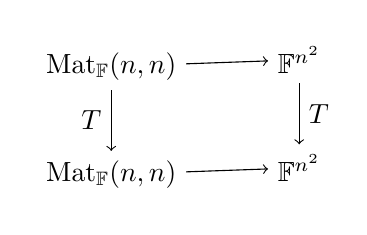
\begin{tikzpicture}
  \matrix (m) [matrix of math nodes, row sep=2em, column sep=3em, minimum width=1em]
  {
    \text{Mat}_{\mathbb{F}}(n,n) & \mathbb{F}^{n^2} \\
    \text{Mat}_{\mathbb{F}}(n,n) & \mathbb{F}^{n^2} \\ 
  };
  \path[->]
  (m-1-1) edge node [auto] {$$} (m-1-2)
          edge node [left] {$T$} (m-2-1)
  (m-1-2) edge node [auto] {$T$} (m-2-2)
  (m-2-1) edge node [auto] {$$} (m-2-2)        
          ;
  \end{tikzpicture} \qquad \, 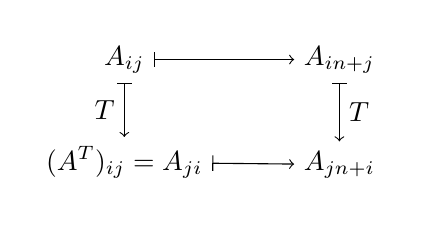
\begin{tikzpicture}
  \matrix (m) [matrix of math nodes, row sep=2em, column sep=3em, minimum width=1em]
  {
A_{ij} & A_{in+j} \\ 
(A^T)_{ij} = A_{ji} & A_{jn+i} \\
  };
  \path[|->]
  (m-1-1) edge node [auto] {$$} (m-1-2)
          edge node [left] {$T$} (m-2-1)
  (m-1-2) edge node [auto] {$T$} (m-2-2)
  (m-2-1) edge node [auto] {$$} (m-2-2)        
          ;
  \end{tikzpicture}
\]

\href{https://classroom.udacity.com/courses/cs344/lessons/77202674/concepts/773153710923}{Transpose Part 2}

Possibly, transpose is a functor.

Consider struct as a category.  In this special case, $\text{Obj}\text{struct} = \lbrace \text{arrays} \rbrace$ (a struct of arrays).  Now this struct already has a hash table for indexing upon declaration (i.e. ``creation''): so this category struct will need to be equipped with a ``diagram'' from the category of indices $J$ to struct: $J\to $ struct.

So possibly
\[
\begin{aligned}
  \text{struct} & \xrightarrow{T} & \text{ array } \\ 
 \text{Obj}\text{Struct} = \lbrace \text{ arrays } \rbrace & \xrightarrow{T} & \text{Obj}\text{array} = \lbrace \text{ struct } \rbrace \\ 
 J\to \text{ struct } & \xrightarrow{T} & J \to \text{ array } 
  \end{aligned}
\]







\href{https://classroom.udacity.com/courses/cs344/lessons/77202674/concepts/787012800923}{Quiz: What Kind Of Communication Pattern}
This quiz made a few points that clarified the characteristics of these so-called communication patterns (amongst the memory?)

\begin{itemize}
  \item map is bijective, and map $:\text{Idx} \to \text{Idx}$
  \item gather - not necessarily surjective
  \item scatter - not necessarily surjective 
  \item stencil - surjective
  \item transpose (see before)
  \end{itemize}




\href{https://classroom.udacity.com/courses/cs344/lessons/77202674/concepts/773153720923}{Parallel Communication Patterns Recap}

\begin{itemize}
\item map - bijective
\item transpose - bijective
\item gather - not necessarily surjective, and is many-to-one (by def.)
\item scatter - one-to-many (by def.) and is not necessarily surjective
\item stencil - several-to-one (not injective, by definition), and is surjective
\item reduce - all-to-one
  \item scan/sort - all-to-all
\end{itemize}

\href{https://classroom.udacity.com/courses/cs344/lessons/77202674/concepts/773153760923}{Programmer View of the GPU}

thread blocks: group of threads that cooperate to solve a (sub)problem

\href{https://classroom.udacity.com/courses/cs344/lessons/77202674/concepts/773153770923}{Thread Blocks And GPU Hardware}

CUDA GPU is a bunch of SMs:

Streaming Multiprocessors (SM)s

SMs have a bunch of simple processors and memory.

Dr. Luebki:
\[
\boxed{ \begin{gathered}
    \text{Let me say that again because it's really important} \\
    \text{GPU is responsible for allocating blocks to SMs}
  \end{gathered}
  }
\]
Programmer only gives GPU a pile of blocks.

\href{https://classroom.udacity.com/courses/cs344/lessons/77202674/concepts/787721730923}{Quiz: What Can The Programmer Specify}

I myself thought this was a revelation and was not intuitive at first:

Given a single kernel that's launched on many thread blocks include $X$, $Y$, the programmer cannot specify the sequence the blocks, e.g. block $X$, block $Y$, run (same time, or run one after the other), and which SM the block will run on (GPU does all this).  

\href{https://classroom.udacity.com/courses/cs344/lessons/77202674/concepts/787981160923}{Quiz: A Thread Block Programming Example}

Open up \verb|hello blockIdx.cu| in Lesson 2 Code Snippets (I got the repository from github, repo name is cs344).

At first, I thought you can do a single file compile and run in Eclipse without creating a new project.  No.  cf. \href{http://stackoverflow.com/questions/17164197/eclipse-creating-projects-every-time-to-run-a-single-file}{Eclipse creating projects every time to run a single file?}.  

%I opened it up in Eclipse with File, Open File (no need to create a new project).

I ended up creating a new CUDA C/C$++$ project from File -> New project, and then chose project type Executable, Empty Project, making sure to include Toolchain CUDA Toolkit (my version is 7.5), and chose an arbitrary project name (I chose cs344single).  Then, as suggested by \href{http://stackoverflow.com/users/3720356/kenny-nguyen}{Kenny Nguyen}, I dragged and dropped files into the folder, from my file directory program.

I ran the program with the ``Play'' triangle button, clicking on the green triangle button, and it ran as expected.  I also turned off Build Automatically by deselecting the option (no checkmark).

\href{https://classroom.udacity.com/courses/cs344/lessons/77202674/concepts/773883100923}{GPU Memory Model}

\[
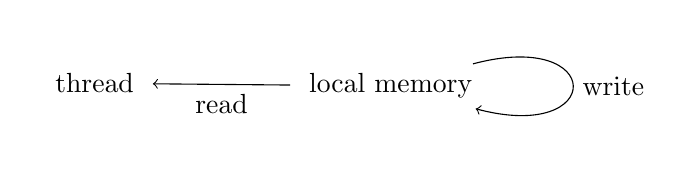
\begin{tikzpicture}
  \matrix (m) [matrix of math nodes, row sep=4em, column sep=5em, minimum width=2em]
  {
\text{ thread } & \text{ local memory } \\
};
  \path[->]
  (m-1-2) edge node [auto] {$\text{read}$} (m-1-1)
  (m-1-2) edge [loop right] node [right] {$\text{write}$} (m-1-2)
  ;
  \end{tikzpicture}
\]

Then consider threadblock $\equiv$  thread block \\
\phantom{Then consider } $\text{Obj}\text{threadblock} \supset \lbrace \text{ threads } \rbrace$ \\
\phantom{Then consider } $\text{FinSet} \xrightarrow{ \text{ threadIdx} } \text{ thread } \in \text{Mor}\text{threadblock}$

\[

\begin{tikzpicture}
  \matrix (m) [matrix of math nodes, row sep=4em, column sep=5em, minimum width=2em]
  {
\text{ threadblock } & \text{ shared memory } \\
};
  \path[->]
  (m-1-2) edge node [auto] {$\text{read}$} (m-1-1)
  (m-1-2) edge [loop right] node [right] {$\text{write}$} (m-1-2)
  ;
  \end{tikzpicture}
\]
$\forall \, $ thread,
\[
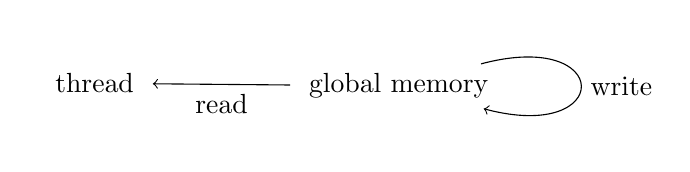
\begin{tikzpicture}
  \matrix (m) [matrix of math nodes, row sep=4em, column sep=5em, minimum width=2em]
  {
\text{ thread } & \text{ global memory } \\
};
  \path[->]
  (m-1-2) edge node [auto] {$\text{read}$} (m-1-1)
  (m-1-2) edge [loop right] node [right] {$\text{write}$} (m-1-2)
  ;
  \end{tikzpicture}
\]

\href{https://classroom.udacity.com/courses/cs344/lessons/77202674/concepts/773883130923}{Synchronization - Barrier}

\href{https://classroom.udacity.com/courses/cs344/lessons/77202674/concepts/785776150923}{Quiz: The Need For Barriers}

3 barriers were needed (wasn't obvious to me at first).  All threads need to finish the write, or initialization, so it'll need a barrier.

While
\begin{lstlisting}
array[idx] = array[idx+1];
  \end{lstlisting}
is 1 line, it'll actually need 2 barriers; first read.  Then write.

So \emph{actually} we'll need to \emph{rewrite} this code:
\begin{lstlisting}
  int temp = array[idx+1];
  __syncthreads();
  array[idx] = temp;
  __syncthreads();
  \end{lstlisting}

kernels have implicit barrier for each.  

\href{https://classroom.udacity.com/courses/cs344/lessons/77202674/concepts/774332060923}{Writing Efficient Programs}

\begin{enumerate}
\item Maximize \emph{arithmetic intensity}
  arithmetic intensity $:= \frac{ \text{ math } }{ \text{ memory }}$
  \end{enumerate}

\href{https://classroom.udacity.com/courses/cs344/lessons/77202674/concepts/774332070923}{video: Minimize Time Spent On Memory}

local memory is fastest; global memory is slower

\[
\text{local} > \text{ shared} >> \text{global} >> \text{CPU}
\]

kernel we know (in the code) is tagged with \verb|__global__|

\href{https://classroom.udacity.com/courses/cs344/lessons/77202674/concepts/814086830923}{quiz: A Quiz on Coalescing Memory Access}

Work it out as Dr. Luebki did to figure out if it's coalesced memory access or not.  


\href{https://classroom.udacity.com/courses/cs344/lessons/77202674/concepts/774332150923}{Atomic Memory Operations}

Atomic Memory Operations

atomicadd atomicmin atomicXOR atomicCAS Compare And Swap



\section{Pointers in C; Pointers in C categorified (interpreted in Category Theory)}

Suppose $v\in \text{ObjData}$, category of data \textbf{Data}, \\
\phantom{ Suppose} e.g. $v\in \text{Int} \in \text{Obj}\mathbf{\text{Type}}$, category of types $\mathbf{\text{Type}}$.

\[
\begin{aligned}
  & \text{Data}  \xrightarrow{ \& } \text{Memory}  \\
  & v \overset{\&}{\mapsto} \& v 
\end{aligned}
\]
with address $\& v \in $ Memory.

With \\
\phantom{With } assignment $pv = \& v$,
\[
\begin{aligned}
  & pv \in \text{Obj}\text{pointer}, \, \text{ category of pointers, pointer} \\ 
  & pv \in \text{Memory} \qquad \, (\text{i.e. not $pv \in \text{Dat}$, i.e. $pv \notin \text{Dat}$})
\end{aligned}
\]

\[
\text{ pointer } \ni pv \overset{ * }{ \mapsto } *pv \in \text{Dat}
\]

\[
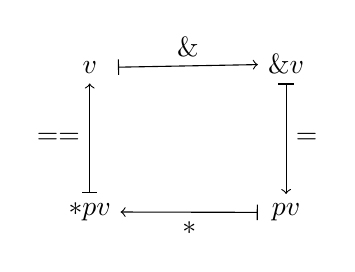
\begin{tikzpicture}
  \matrix (m) [matrix of math nodes, row sep=4em, column sep=5em, minimum width=2em]
  {
    v & \& v \\
    *pv & pv \\
};
  \path[|->]
  (m-1-1) edge node [auto] {$\&$} (m-1-2)
  (m-1-2) edge node [right] {$=$} (m-2-2)
  (m-2-2) edge node [auto] {$*$} (m-2-1)
  (m-2-1) edge node [left] {$==$} (m-1-1)
  ;
  \end{tikzpicture}
\qquad \, 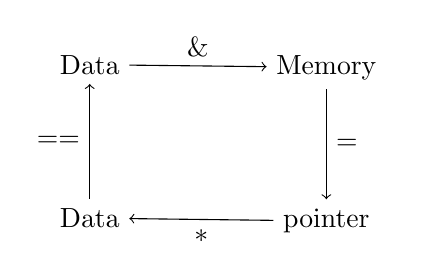
\begin{tikzpicture}
  \matrix (m) [matrix of math nodes, row sep=4em, column sep=5em, minimum width=2em]
  {
    \text{Data} & \text{Memory} \\
    \text{Data} & \text{pointer} \\
};
  \path[->]
  (m-1-1) edge node [auto] {$\&$} (m-1-2)
  (m-1-2) edge node [right] {$=$} (m-2-2)
  (m-2-2) edge node [auto] {$*$} (m-2-1)
  (m-2-1) edge node [left] {$==$} (m-1-1)
  ;
  \end{tikzpicture}
\]

Examples.  Consider \verb|passfunction.c| in Fitzpatrick \cite{Fitz}.

Consider the type \verb|double|, \verb|double| $\in \text{Obj}\text{Types}$.  \\
\phantom{ Consider } $\text{fun1, fun2} \in \text{Mor}\text{Types} \qquad \, \text{ namely }$ \\
\phantom{ Consider } $\text{fun1, fun2} \in \text{Hom}(\text{double},\text{double}) \equiv \text{Hom}_{\text{Types}}(\text{double},\text{double})$

Recall that
\[
\begin{aligned}
  & \text{ pointer } \xrightarrow{ * } \text{ Dat } \\ 
  & \text{ pointer } \xrightarrow{ \& } \text{ Memory }
\end{aligned}
\]
$*, \&$ are functors with domain on the category pointer.

Pointers to functions is the ``extension'' of functor $*$ to the codomain of $\text{Mor}\text{Types}$:

\[
\begin{aligned}
  & \text{ pointer} & \xrightarrow{ * } \text{Mor}\text{Types} \\ 
  & \text{ fun1 } & \overset{*}{ \mapsto } *\text{fun}1 \in \text{Hom}_{\text{Types}}(\text{double},\text{double})
  \end{aligned}
\]

\[
 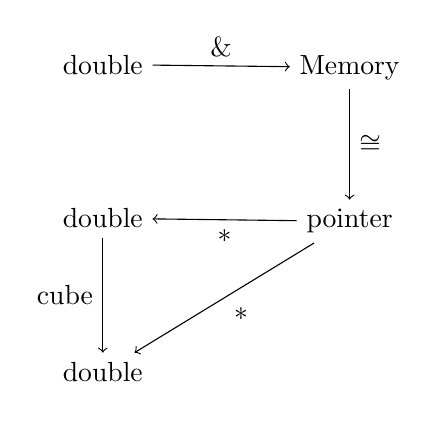
\begin{tikzpicture}
  \matrix (m) [matrix of math nodes, row sep=4em, column sep=5em, minimum width=2em]
  {
    \text{double} & \text{Memory} \\
    \text{double} & \text{pointer} \\
    \text{double} & \\ 
  };
  \path[->]
  (m-1-1) edge node [auto] {$\&$} (m-1-2)
  (m-1-2) edge node [right] {$\cong$} (m-2-2)
  (m-2-2) edge node [auto] {$*$} (m-2-1)
  edge node [auto] {$*$} (m-3-1)
  (m-2-1) edge node [left] {$\text{cube}$} (m-3-1)
  ;
 \end{tikzpicture} \qquad \qquad \,
  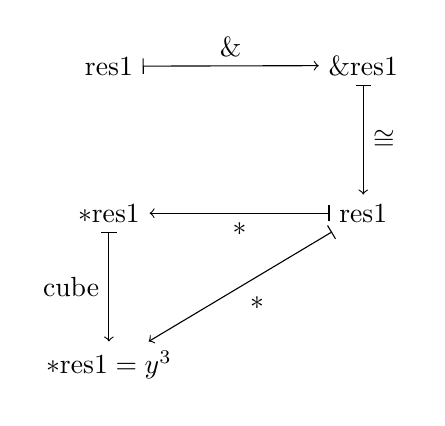
\begin{tikzpicture}
  \matrix (m) [matrix of math nodes, row sep=4em, column sep=5em, minimum width=2em]
  {
    \text{res1} & \&\text{res1} \\
    *\text{res1} & \text{res1} \\
    *\text{res1} = y^3 & \\ 
  };
  \path[|->]
  (m-1-1) edge node [auto] {$\&$} (m-1-2)
  (m-1-2) edge node [right] {$\cong$} (m-2-2)
  (m-2-2) edge node [auto] {$*$} (m-2-1)
  edge node [auto] {$*$} (m-3-1)
  (m-2-1) edge node [left] {$\text{cube}$} (m-3-1)
  ;
  \end{tikzpicture}
\]

It's unclear to me how \verb|void cube| can be represented in terms of category theory, as surely it cannot be represented as a mapping (it acts upon a functor, namely the $*$ functor for pointers).  It doesn't return a value, and so one cannot be confident to say there's explicitly a domain and codomain, or range for that matter.

But what is going on is that
\[
\begin{gathered}
  \text{ pointer }, \text{ double } , \text{ pointer } \xrightarrow{ \text{ cube } } \text{ pointer }, \text{ pointer } \\ 
  \text{fun}1, x , \text{res}1 \overset{\text{cube}}{\mapsto} \text{fun}1, \text{res}1
\end{gathered}
\]
s.t. $*\text{res}1 = y^3=(*\text{fun}1(x))^3$


So I'll speculate that in this case, \verb|cube| is a functor, and in particular, is acting on $*$, the so-called deferencing operator:
\[
\begin{gathered}
  \text{ pointer } \xrightarrow{ * } \text{float} \in \text{Data} \\
  \text{ res}1 \overset{*}{\mapsto} *\text{res}1
\end{gathered} \xrightarrow{ \text{ cube } } \begin{gathered}
  \text{ pointer } \xrightarrow{ \text{cube}(*) } \text{float} \in \text{Data} \\
  \text{ res}1 \overset{\text{cube}(*)}{\mapsto} \text{cube}(*\text{res}1)=y^3
\end{gathered}
\]


\subsubsection{Need a CUDA, C, C$++$, IDE?  Try Eclipse!}

This website has a clear, lucid, and pedagogical tutorial for using Eclipse: \href{https://www.fayewilliams.com/2011/06/28/creating-your-first-c-program-in-eclipse/}{	
Creating Your First C++ Program in Eclipse}.  But it looks like I had to pay.  Other than the well-written tips on the webpage, I looked up stackexchange for my Eclipse questions (I had difficulty with the Eclipse documentation).  




\end{multicols*}
\begin{thebibliography}{9}
\bibitem{HTF2009}
Trevor Hastie, Robert Tibshirani, Jerome Friedman.   \textbf{The Elements of Statistical Learning: Data Mining, Inference, and Prediction}, Second Edition (Springer Series in Statistics) 2nd ed. 2009. Corr. 7th printing 2013 Edition.  ISBN-13: 978-0387848570.  \url{https://web.stanford.edu/~hastie/local.ftp/Springer/OLD/ESLII_print4.pdf}

\bibitem{CS2013}
Jared Culbertson, Kirk Sturtz.  \emph{Bayesian machine learning via category theory}.  \href{http://arxiv.org/abs/1312.1445}{arXiv:1312.1445} [math.CT]

\bibitem{CS344}
John Owens.  David Luebki.  \emph{Intro to Parallel Programming}.  \emph{CS344}.  \textbf{\href{https://www.udacity.com/}{Udacity}}  
  
\url{http://arxiv.org/abs/1312.1445} Also, \url{https://github.com/udacity/cs344}  

\bibitem{CS229}
CS229 Stanford University.  \url{http://cs229.stanford.edu/materials.html}


\bibitem{Fitz}
Richard Fitzpatrick.  ``Computational Physics.''  \url{http://farside.ph.utexas.edu/teaching/329/329.pdf}




\end{thebibliography}

\end{document}
